\newpage
\section{Aufgabenstellung 3}

\subsection{Ausgangssituation}
Sie sind Teil eines Qualitätssicherungsteams in einem fiktiven Unternehmen, das eine E-Commerce-Plattform betreibt. Die Plattform bietet Kameraprodukte an, nutzt KI-gestützte Produktsuche, integriert verschiedene Backend-Systeme (z. B. SAP, AWS, NetSuite, HubSpot) und führt den Nutzer durch einen komplexen, serviceorientierten Kaufprozess.Ein zentraler Bestandteil dieses Systems ist der in der beigefügten Prozessgrafik dargestellte End-to-End-Ablauf, vom Website-Besuch bis zur finalen Mail-Bestätigung. Die Architektur umfasst APIs, externe Services, Cloud-Provisionierung und ERP-Integration.

\subsection{Ziel}
\textit{Erarbeiten Sie als Gruppe eine ganzheitliche Teststrategie für dieses System. Die Strategie soll praktikabel sein, typische Herausforderungen im DevOps-Umfeld adressieren und die Integration verschiedener Testebenen, Tools und Umgebungen berücksichtigen.}

\subsection{Bearbeitungsschwerpunkte}
\textit{Bitte erarbeiten Sie eine Ausarbeitung (max. 6 Seiten + Anhang), in der Sie folgende Punkte behandeln:}

\subsubsection{1. Testumgebungsstabilisierung}
\begin{itemize}
    \item \textit{Wie stellen Sie in der Entwicklungs- und Integrationsphase eine stabile Testumgebung sicher, insbesondere angesichts externer Systeme (SAP, AWS, GPT, HubSpot etc.)?}
    \item \textit{Wie kann Service-Virtualisierung oder Mocking zum Einsatz kommen?}
    \item \textit{Welche Datenanforderungen bestehen (z. B. synthetische Testdaten, Daten-Maskierung)?}
\end{itemize}
Für unsere E-Commerce-Plattform mit ihren vielfältigen Integrationen (SAP, AWS, GPT, HubSpot) setzen wir auf:
\begin{itemize}
    \item \textbf{Infrastruktur als Code (IaC):} Wir nutzen Terraform/CloudFormation, um isolierte Testumgebungen automatisiert zu erstellen und zu verwalten.
    \item \textbf{Umgebungsmodellierung:} Jede Testumgebung wird mit ihren Komponenten, Konfigurationen und Testdaten dokumentiert, für bessere Transparenz und Kontrolle.
    \item \textbf{Containerisierung:} Kubernetes-Namespaces für kurzlebige, isolierte Testumgebungen.
    \item \textbf{Sandbox-Accounts:} Dedizierte Test-Accounts für Cloud-Dienste verhindern Konflikte zwischen Teams.
\end{itemize}
Zusammenfassend isolieren wir und verwalten die Infrastruktur mittels Infrastructure as Code (z.\,B. Terraform/CloudFormation) und nutzen dedizierte Sandbox-Accounts, um Konflikte zu vermeiden. Service-Virtualisierung ist eine zentrale Strategie die im nächsten Abschnitt beschrieben wird. Für eine beispielhafte Darstellung der Umgebung siehe Abbildung~\ref{fig:deployment}).
\begin{figure}[h!]
\centering
\caption{Deployment-Diagramm: Virtuelle Testumgebungen via IaC}
    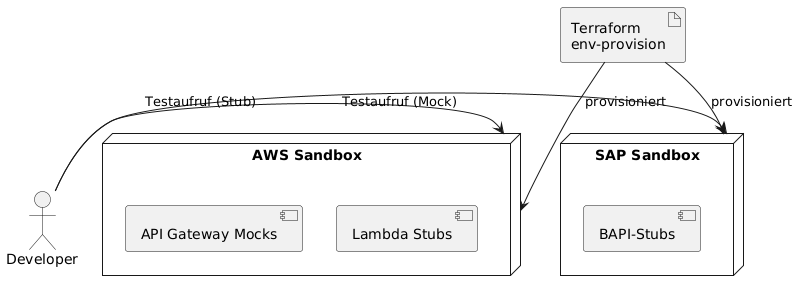
\includegraphics[width=0.8\textwidth]{fig/stubing.png}
    \label{fig:deployment}
\end{figure}
\paragraph{Service-Virtualisierung und Mock-Ansätze}
Service-Virtualisierung ist entscheidend, wenn externe Systeme nicht verfügbar oder instabil sind:
\begin{itemize}
    \item \textbf{REST/HTTP-Interfaces:} WireMock oder Mountebank für die Simulation von REST-APIs.
    \item \textbf{Cloud-APIs:} AWS LocalStack für lokale Emulation von AWS-Services.
    \item \textbf{ERP-Integration:} Virtualisierung von SAP BAPIs und speziellen Schnittstellen.
    \item \textbf{API-Gateway:} Nutzung von AWS API Gateway zur Erstellung von Mock-Endpunkten.
\end{itemize}
Wenn abhängige Systeme (ERP oder externe APIs) instabil oder nicht verfügbar sind, simulieren Virtualisierungstools realistische Interaktionen. Open-Source-Lösungen wie WireMock oder Mountebank stubben REST-/HTTP-Schnittstellen, während Cloud-Tools (z.\,B. AWS LocalStack) Cloud-APIs lokal emulieren. Der Ablauf ist in Abbildung~\ref{fig:sequence} dargestellt.\begin{figure}[h!]
\centering
\caption{Sequenzdiagramm: Service-Virtualisierung mit WireMock}
    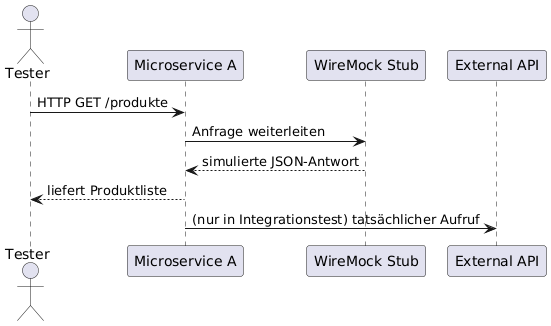
\includegraphics[width=0.8\textwidth]{fig/servicevirti.png}
    \label{fig:sequence}
\end{figure}

\newpage
\paragraph{Testdatenmanagement}
Um konsistente und compliance-konforme Tests zu gewährleisten:
\begin{itemize}
    \item \textbf{Datenmaskierung:} Ersetzen von PII mit realistischen fiktiven Werten unter Beibehaltung der referentiellen Integrität.
    \item \textbf{Synthetische Daten:} Künstliche Datensätze für Spezialfälle und Randszenarien.
    \item \textbf{Hybridansatz:} Maskierte Produktionsdaten für Basistests, ergänzt durch synthetische Daten für Edge-Cases.
    \item \textbf{API-Integration:} CI/CD-Pipeline kann Testdaten über APIs auffrischen, zurücksetzen oder klonen.
\end{itemize}
\subsubsection{2. Testarten und Abdeckung}
\begin{itemize}
    \item \textit{Welche Testarten (z. B. Unit-, API-, Integrations-, E2E-, Load-, Performance-, Security-tests) sind erforderlich, um:}
    \begin{itemize}
        \item \textit{die funktionalen Anforderungen abzudecken?}
        \item \textit{nicht-funktionale Anforderungen wie Performance, Security, Verfügbarkeit und Datenintegrität zu prüfen?}
    \end{itemize}
    \item \textit{Wo und wie werden diese Tests innerhalb der CI/CD-Pipeline ausgeführt?}
\end{itemize}

\paragraph{Funktionale Tests}
Zur Abdeckung funktionaler Anforderungen setzen wir folgende Testtypen ein:
\begin{itemize}
    \item \textbf{Unit-Tests:} Für einzelne Module/Services, laufen bei jedem Commit.
    \item \textbf{API-Tests:} Validierung jeder Microservice-Schnittstelle gegen ihre Spezifikation (mit JUnit, pytest oder Postman/Newman).
    \item \textbf{Integrationstests:} Testen zusammenhängender Dienste (z.B. Inventarsynchronisation von SAP zu NetSuite).
    \item \textbf{End-to-End-Tests:} Simulation realer Benutzerszenarien (Produktsuche, Checkout etc.) mit Selenium, Cypress oder Playwright.
\end{itemize}
\paragraph{Nicht-funktionale Tests}
Zur Prüfung von Performance, Security, Verfügbarkeit und Datenintegrität verwenden wir:
\begin{itemize}
    \item \textbf{Performance/Last-Tests:} Apache JMeter oder Gatling zur Simulation von Verkehrsspitzen und Messung der Skalierbarkeit.
    \item \textbf{Security-Tests:} Kombination aus statischer (SAST) und dynamischer (DAST) Analyse mit Tools wie SonarQube, Snyk oder OWASP ZAP.
    \item \textbf{Verfügbarkeitstests:} Monitoring der Systemverfügbarkeit unter verschiedenen Lastbedingungen.
    \item \textbf{Datenintegritätstests:} Validierung der Datenkonsistenz zwischen SAP, NetSuite und AWS.
\end{itemize}
\subsubsection{3. Testeffizienz und Wartbarkeit}
\begin{itemize}
    \item Wie strukturieren Sie Tests, um gezielt auf Systemveränderungen (z. B. SAP-Upgrade) reagieren zu können?
    \item Wie nutzen Sie z. B. Impact Analysis, modulare Architekturen oder risikobasiertes Testen, um Wiederverwendbarkeit und Selektivität zu ermöglichen?
\end{itemize}

\subsubsection{4. Reporting \& Testtransparenz}
\begin{itemize}
    \item Wo und wie sollen Testergebnisse dokumentiert und ausgewertet werden (z. B. Dashboards, Logs, automatisierte Reports)?
    \item Wer sind die Stakeholder für das Reporting (Dev, QA, Ops, Management)?
\end{itemize}

\subsubsection{5. Toolauswahl und Integration}
\begin{itemize}
    \item Welche Testtools (open source und/oder kommerziell) schlagen Sie für die Umsetzung vor für z. B.:
    \begin{itemize}
        \item Testautomatisierung
        \item Performance-Testing
        \item Service-Virtualisierung
        \item Testdatenmanagement
        \item Reporting \& Testmanagement
    \end{itemize}
\end{itemize}

\subsection{Teamarbeit \& Rollenverteilung}
Versucht in der Ausarbeitung die folgenden Rollen einzunehmen:
\begin{itemize}
    \item QA-Architekt: übergreifendes Testkonzept \& Architektur
    \item Testanalyst: Spezifikation von Testfällen und Daten
    \item Tool-Integrator: Toolauswahl \& CI/CD-Verknüpfung
\end{itemize}
Die Aufteilung ist eine Empfehlung, aber keine Pflicht.

\subsection{Abzugebende Materialien}
\begin{itemize}
    \item Schriftliches Konzept (PDF, max. 6 Seiten ohne Anhang)
    \item Architektur- oder Ablaufdiagramm(e) zur Teststrategie
    \item Tabelle mit empfohlener Tool-Landschaft
\end{itemize}

\subsection{Vorgesehene Bearbeitungsdauer}
Gesamt in etwa 5 Stunden pro Person.

\subsection{Lernziele}
\begin{itemize}
    \item Eine effektive Teststrategie im Kontext von DevOps
    \item Den Einsatz moderner Testtools konzeptionell bewerten
    \item Risiken in komplexen Integrationslandschaften erkennen und adressieren
    \item Testgetriebene CI/CD-Prozesse planen und visualisieren
\end{itemize}
